

\documentclass[letterpaper]{article}

\usepackage{hyperref}
\usepackage{geometry}
\usepackage{xspace}
\usepackage{graphicx}
\usepackage[T1]{fontenc}
\usepackage[sc,osf]{mathpazo}
\usepackage{amsmath}

\def\name{Jose Ignacio Castelli}
\def\footerlink{https://github.com/JicLotus/CV}

% PDF metadata
\hypersetup{
  colorlinks = true,
  urlcolor = black,
  pdfauthor = {\name},
  pdfkeywords = {android, software development, algorithms, computer science, mathematics},
  pdftitle = {\name: Curriculum Vitae},
  pdfsubject = {Curriculum Vitae},
  pdfpagemode = UseNone
}

\geometry{
  body={6.5in, 8.5in},
  left=1.0in,
  top=1.25in
}

% Page headers
\pagestyle{myheadings}
\markright{\name}
\thispagestyle{empty}

% Custom section fonts
\usepackage{sectsty}
\sectionfont{\rmfamily\mdseries\Large}
\subsectionfont{\rmfamily\mdseries\itshape\large}

% Don't indent paragraphs.
\setlength\parindent{0em}

% Make lists without bullets
\renewenvironment{itemize}{
  \begin{list}{}{
    \setlength{\leftmargin}{1.5em}
  }
}{
  \end{list}
}

\newenvironment{no-indent-itemize}{
  \begin{list}{}{
    \setlength{\leftmargin}{0em}
  }
}{
  \end{list}
}

\def\tilde{$\scriptstyle\sim$}
\def\bullet{$\circ$\xspace}

\begin{document}

{\huge \name}



\bigskip
\begin{minipage}{0.45\linewidth}
  \begin{tabular}{llll}
    
    
    Email: & \href{mailto:joseignaciocastelli92@gmail.com}{\tt joseignaciocastelli92@gmail.com} \\
     
    
    Github: &\href{http://github.com/jiclotus}{\tt http://github.com/jiclotus}\\
    
    Linkedin: &\href{https://www.linkedin.com/in/jose-ignacio-castelli-138763b0/}{\tt https://www.linkedin.com/in/jose-ignacio-castelli-138763b0/}\\
    
    Languages: & English, Spanish\\
    Birth Date: & \textsc{07-18-1992} \\
    Citizenships: & Italian, Argentinian
    
  \end{tabular}
\end{minipage}


\hfill 
\smash{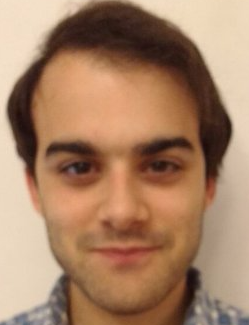
\includegraphics[width=3cm,height=3.5cm]{profilePic.png}}


\section*{Education}
\begin{no-indent-itemize}
  \item\bullet When I was twenty-four, I hold a degree in Software Engineering from University of Buenos Aires 2011-2016 ( It is a 6-year university course equivalent to \textbf{BS+MS}) 
  \item\bullet GPA: 7.11 of 10.0
\end{no-indent-itemize}


\section*{Employment}
\begin{no-indent-itemize}

    \item\textsc{Sr Software Engineer at RS} | Jan 2017 - Present
    \begin{itemize}
    \item\bullet I'm working on a Billing management system for Supervielle Bank. It is a very interesting experience because the infrastructure is quite big
    \item\bullet In three months I learned the totality of source code and I can do whatever business is required. I have done a lot of things related to the programming tasks, for example, I developed a PDF parser for AFIP bills.
    \item\bullet We use Jenkins for CI and scripts in PowerShell for automatic deploy
    \item\bullet  Scrum, C\# , .Net framework , MSSQL, SOAP, and JS.
    \end{itemize}


    \item \textsc{Software Developer at Celulosa Baradero SA} | Sep 2015 - May 2016
    \begin{itemize}
    \item\bullet  When I was twenty-two I developed a management software. This project was to control coils for a recycling plant. With this software, you can manage the coil stock with a cell phone through reading QR code.
    \item\bullet
    \href{https://github.com/JicLotus/Control-Sistematico-QR}{https://github.com/JicLotus/Control-Sistematico-QR}
    \item\bullet Scrum, C\# .Net FrameWork, Mysql, Php, \textbf{JAVA} and Android.
    \end{itemize}
    
    
    \item\textsc{Game Developer at InmortalAO} | Dec 2011 - Jul 2014
    \begin{itemize} 
    \item\bullet
    When I was twenty I had a 2D game with 167 players simultaneously. The last version was developed in C\# and \textbf{C++}. The users uploaded game plays on YouTube and you can check it.
    \item\bullet \href{https://www.facebook.com/InmortalAO/}{https://www.facebook.com/InmortalAO/}
    \item\bullet Dx11, \textbf{C++}, C\# .Net , MongoDB and Mysql
    \end{itemize}
    
    
    \item \textsc{Game Developer at LocalStrike and NRG Games} | Jan 2007 - Jul 2008
    \begin{itemize} 
    
    \item\bullet
    When I was fifteen I had a sponsor for a 2D game that I developed and managed. This game was a model of an Argentine game called Argentum Online. We were a group of eight persons working on that project. It was online with 110 players simultaneously.
    \item\bullet The first sponsor name was LocalStrike. They gave me a free server connection. My Second sponsor was NRG Games.
    \item\bullet Dx8 and Mysql
    \end{itemize}


\end{no-indent-itemize}


\section*{Projects}
\begin{no-indent-itemize}
    
    \item \textsc{3D WebGL Graphic Scene} | May 2016 - Jun 2016
    \begin{itemize}
    \item\bullet It is a 3D graphic scene. It was developed in WebGL and Java Script. The 3D models were developed without any model external library(such as ThreeJS). The location of each vertex point in the graphic scene was positioned mathematically.
    \end{itemize}
    \begin{itemize}
    \item \href{https://github.com/JicLotus/3DGraphicScene}{https://github.com/JicLotus/3DGraphicScene}
    
    \end{itemize}

    \item \textsc{C++/Android Dropbox Open Source} | Aug 2015 - Dec 2015
    \begin{itemize}
        \item\bullet It's Dropbox open source for Android.
        \item\bullet The web server was developed in RocksDB in \textbf{C++} language.
        \end{itemize}    
    \begin{itemize}
        \item \href{https://github.com/JicLotus/Dropbox-source}{https://github.com/JicLotus/Dropbox-source}
    \end{itemize}

    \item \textsc{Capacitive touch sensors} |  Apr 2015 - Jul 2015

    \begin{itemize}
        \item\bullet This project consists in the implementation of two capacitive touch sensors using an Atmega88pa microcontroller. These sensors were used for the control of intensity of a 12 Voltage(voltash) light.
         
         \href{https://github.com/JicLotus/Capacitive-Sensor}{https://github.com/JicLotus/Capacitive-Sensor}
    \end{itemize}

\end{no-indent-itemize}

\section*{Skills}
\begin{no-indent-itemize}
    
    \item\textsc{Sr Experience}:
    \begin{itemize}
        \item\bullet \underline{Languages}: C\# .Net Framework, \textbf{C++}, C, SQL
        \item\bullet \underline{DB}: Mysql, MSSql
    \end{itemize} 
    \item \textsc{SSr Experience}:
    \begin{itemize}
        \item\bullet \underline{Languages}: \textbf{JAVA}, Python, Php, Android and JavaScript
        \item\bullet \underline{DB}: MongoDB and RocksDB
        \item\bullet \underline{Video Games Api}: DirectX, OpenGL, WebGL, SDL, XNA
        \item\bullet \underline{Frameworks}: Laravel
        \item\bullet \underline{Web Servers}: IIS and Apache.
    \end{itemize}     
    \item \textsc{Jr Experience}:
    \begin{itemize}
        \item\bullet \underline{Languages}: \textbf{GO}
    \end{itemize}      

\end{no-indent-itemize}



\section*{Extracurriculars}
\begin{no-indent-itemize}
    \item\bullet Since I was thirteen years old I have been developing video games and company management systems in different languages. 
    \item\bullet I love playing the drums in my free time. I've played them since I was thirteen years old
\end{no-indent-itemize}






\bigskip
\begin{center}
  \begin{footnotesize}
    Last updated: \today \\
    \href{\footerlink}{\texttt{\footerlink}}
  \end{footnotesize}
\end{center}

\end{document}
